\section{Guth-Maynard's proof of Large Values of Dirichlet Polynomials}
In June 2024, Guth and Maynard published an improvement of the large values of Dirichlet polynomails estimate at $\sigma\in[7/10,8/10]$.
\begin{theorem}[Guth-Maynard Large Values Estimate]
    Let $(b_n)$ be a sequence of complex numbers such that $|b_n|\leq 1$ for all $n$, and $W=\{t_j\}_{j=1}^{|W|}$ be a $1$-separated set $\subseteq [0,T]$, such that \[
    \left|\sum_{n\sim N}b_n n^{it_j}\right|\geq V
    \]
    for each $t_j\in W$. Then \[
    |W|\lesssim N^2V^{-2}+N^{18/5}V^{-4}+TN{12/5}V^{-4}.
    \]
\end{theorem}
Let us compare this bound to Lemma \ref{halasz}, which states \[
|W|\lesssim N^2V^{-2}+TN^4V^{-6}.
\]
In the critical case $V=N^{3/4}, N\leq T^{5/6-\epsilon}$, the original bound will give \[
|W|\lesssim N^2N^{-3/2}+TN^4N^{-9/2}\lesssim N^{1/2}+ TN^{-1/2}\lesssim TN^{-1/2},
\]
while the bound by Guth and Maynard gives \[
|W|\lesssim N^2N^{-3/2}+N^{18/5}N^{-3}+TN^{12/5}N^{-3}\lesssim N^{1/2}+TN^{-3/5}\lesssim TN^{-3/5}.
\]
\subsection{Outline and Sketch of proof}
%\node[label=above/below/etc:{label}] (x) {}
The structure of the proof can be broken down as follows: We first notice that $|W|$ is bounded by the operator norm of a matrix $M$. This operator norm, using results from linear algebra, is bounded by the trace. Applying Poisson summation on the trace gives $4$ terms that are separately handled, which we will name $S_0$ to $S_3$. We will see that $S_0$ gives the `main term' that is consistent with the density hypothesis, $S_1$ is negligible, $S_2$ is bounded by a theorem by Heath-Brown, which we state below. 
\begin{theorem}[Heath-Brown]
    \label{heathbrown}
    Let $\mathcal{S}=\{(t_j,\chi_j)\}$ be one-separate, primitive characters of modulus $q$. Then 
    \[
        \sum_{\substack{(t_1,\chi_1)\\(t_2,\chi_2)}}\left|\sum_{n=1}^{N} b_n n^{-i(t_1-t2)}\chi_1\bar{\chi}_2(n)\right|^2 \lesssim  |\mathcal{S}|N^2+ |\mathcal{S}|^2N + |\mathcal{S}|^{5/4}(qT)^{1/2}N.
    \]
\end{theorem}
Finally, the most tricky term, $S_3$ is a summation over a three-dimensional lattice. We will see that $S_3$ is bounded by what is known as the \textit{additive energy} of the set $W$, defined by\[
    E(W)\defeq \#\{t_1,t_2,t_3,t_4\in W : |t_1+t_2-t_3-t_4|\ll T^\epsilon\}.
\]
This term describes the `additive structure' of $W$.
We see that $E(W)$ is bounded below by $|W|^2$, as the condition is satisfied when $t_1=t_3$ and $t_2=t_4$. Moreover, since $W$ is $1-separated$, the choice of $t_1,t_2,t_3$ fixes $O(1)$ choices for $t_4$, so $E(W)$ is bounded above by $|W|^3$. In the extreme case that the additive structure of $W$ is high, such as when $t_j=j\alpha$ for a constant $\alpha$, the energy of the set is $O(|W|^3)$. This definition naturally arrises from taking the fourth moment of the function \[
R(v)\defeq\sum_{t\in W} v^{it}.
\] 
This gives us \[
R(v)^4=\sum_{t_1,t_2,t_3,t_4\in W}v^{i(t_1+t_2-t_3-t_4)}.
\]

The naive choice $E(W)\leq W^3$ is slightly too loose to beat the Ingham-Huxley bound. However, an orthogonal bound can be found for $E(W)$ based on Heath-Brown's theorem. We give a quick sketch below. In the next chapter, we will give a full proof of the generalized statement of the theorem that considers primitive Dirichlet characters mod $q$. The proof of Guth-Maynard can be recovered by using the special case $q=1$.
\subsubsection*{0. Setup}
First, as in the theorem, we let $(b_n)$ be a sequence of complex numbers such that $|b_n|\leq 1$ for all $n$, \[
D_n(t)\defeq \sum_{n\sim N}b_n n^{it},
\] $W=\{t_j\}_{j=1}^{|W|}$ be a $T^\epsilon$-separated set $\subseteq [0,T]$, such that \[
\left|D_n(t_j)\right|\geq V
\]
for each $t_j\in W$. Notice that we now let the set be $T^\epsilon$ separated for $\epsilon>0$. This means that we will give up a factor of $T^\epsilon$ in the final bound, but this makes many computations cleaner as this $T^\epsilon$ dominates the log factors. Moreover, we can introduce a bump function $\omega$ with support in $[1,2]$ to localize the summation, and rewrite \[
    D_n(t_j)=\sum_{n}\omega\left(\frac{n}{N}\right)b_n n^{it_j}.
\]
This is added for the Poisson summation in step $3$.
\subsection*{1. Bounding $|W|$ with operator norm}
We view $\vec{b}=(b_n)_{n\sim N}$ as a $N$-dimensional vector, and consider the $|W|\times N$ matrix, indexed by $j$ from $1$ to $|W|$ and $n\sim N$,\[
    M_{j,n}=n^{it_j}= \omega\left(\frac{n}{N}\right)n^{i t_j}.
\]
\begin{figure} [t]
    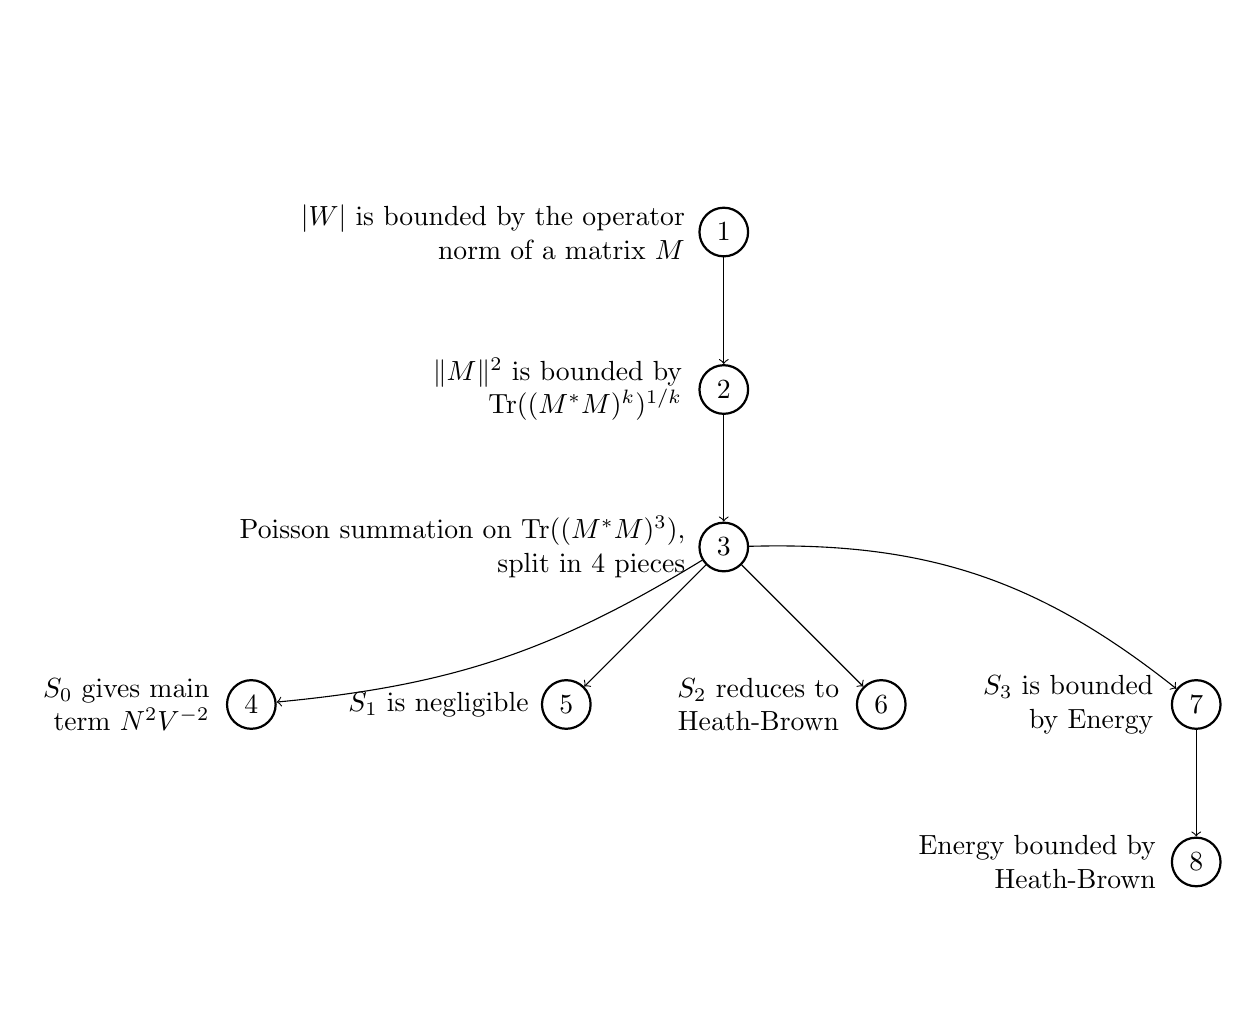
\begin{tikzpicture}
        \begin{scope}[every node/.style={circle,thick,draw}]
            \node [label={[align=right]left:{$|W|$ is bounded by the operator\\ norm of a matrix $M$}}](A) at (0,0) {1};
            \node [label={[align=right]left:{$\|M\|^2$ is bounded by \\$\textrm{Tr}((M^*M)^k)^{1/k}$}}](B) at (0,-2) {2};
            \node [label={[align=right]left:{Poisson summation on $\textrm{Tr}((M^*M)^3)$,\\split in $4$ pieces}}](C) at (0,-4) {3};
            \node [label={[align=right] left:{$S_0$ gives main \\ term $N^2V^{-2}$}}](D) at (-6,-6) {4};
            \node [label={[align=right] left:{$S_1$ is negligible}}](E) at (-2,-6) {5};
            \node [label={[align=right] left:{$S_2$ reduces to\\ Heath-Brown}}](F) at (2,-6) {6};
            \node [label={[align=right] left:{$S_3$ is bounded\\ by Energy}}](G) at (6,-6) {7};
            \node [label={[align=right]left:{Energy bounded by \\ Heath-Brown}}](H) at (6,-8) {8};
        \end{scope}
        %\draw [dotted] (a) --  (b);
        \draw [->](A) -- (B);\draw [->](B) -- (C);
        \path [->](C) edge [bend left =13](D); \draw [->](C) -- (E); \draw [->](C) -- (F); \path [->](C) edge[bend left =20] (G);
        \draw[->] (G)--(H);
        %\draw (a) -- node[midway, below left]{1}(d) -- node[midway, below right]{2}(b);
        %\draw (a)-- node[midway, above left]{2} (c) --node[midway, above right]{1}(b);
\end{tikzpicture}
\caption{Graphical representation of Guth-Maynard proof outline}
\end{figure}
Then we can view the $j$-th entry of the product $M\vec{b}$ as $D_n(t_j)$. In other words \[
|M\vec{b}|^2\geq V^2{|W|}.
\]
However, we can bound $|M\vec{b}|$ using the operator norm of $M$ and $|b_n|\leq 1$ to get\[
    |M\vec{b}|^2\leq \|M\|^2|\vec{b}|^2 \leq \|M\|^2 N.
\]
Combined with the previous inequality, we get \begin{equation}
    \label{basicineq}
|W|\leq \|M\|^2 NV^{-2}.
\end{equation}

\subsubsection*{2. Bounding $\|M\|$}
An immediate way to proceed is to note that $\|M\|^2$ is the largest eigenvalue of $MM^*$, which in turn is bounded by sum of eigenvalues which is the trace of $M^*M$. However, this is somewhat inefficient. Consider $N$-dimensional vector that enumerates through the eigenvalues $(\lambda_n)$ of $MM^*$, so that the trace will be the $L_1$ norm of this vector. In principle, we would like the $L_{\infty}$ norm of this vector, so we can try to take $L_k$ norms of this vector for big $k$ to get close to $L_\infty$. Using an eigenbasis for $MM^*$, we can see that the $L_k$ norm is represented by \[
\left(\sum_{n\sim N}\lambda_n ^ {k}\right)^{1/k}= \textrm{Tr}((MM^*)^k)^{1/k}.
\]
We take $k=3$, which is the highest power we can afford given the tools at our disposal. This gives

\begin{equation}
    \label{traceineq}
    |W|\leq \textrm{Tr}((MM^*)^3)^{1/3} NV^{-2}.
\end{equation}

\subsubsection*{3. Expansion of $\rm{Tr}((MM^*)^3)$}
We first compute 

\begin{align*}
    (MM^*)_{n_1,n_2} = \sum_{t\in W} \omega\left(\frac{n_1}{N}\right)\omega\left(\frac{n_2}{N}\right)
    n_1^{-it_j}n_2^{it_j}
\end{align*}
so that\begin{align*}
    \textrm{tr}((M^*M)^3)=& \sum_{t_1,t_2,t_3\in W}\sum_{n_1,n_2,n_3\sim N} 
    \omega\left(\frac{n_1}{N}\right)^2\omega\left(\frac{n_2}{N}\right)^2\omega\left(\frac{n_3}{N}\right)^2 n_1^{i(t_1-t_3)}
   n_2^{i(t_2-t_1)}
    n_3^{i(t_3-t_2)}\\=& \sum_{t_1,t_2,t_3\in W}\sum_{n_1,n_2,n_3} 
    \omega\left(\frac{n_1}{N}\right)^2\omega\left(\frac{n_2}{N}\right)^2\omega\left(\frac{n_3}{N}\right)^2 \left(\frac{n_1}{N}\right)^{i(t_1-t_3)}
    \left(\frac{n_2}{N}\right)^{i(t_2-t_1)}
    \left(\frac{n_3}{N}\right)^{i(t_3-t_2)}.
\end{align*}
Let $h_t(u)\defeq \omega(u)^2 u^{it}$, we can apply Poisson summation in the inner integral over $n_1,n_2,n_3$ to get 
\begin{equation}\label{poissongm}
    \rm{tr}((M^*M)^3)= N^3\sum_{t_1,t_2,t_3\in W}\sum_{m_1,m_2,m_3}  \hat{h}_{t_1-t_3}(Nm_1)\hat{h}_{t_2-t_1}(Nm_2)\hat{h}_{t_3-t_2}(Nm_3).
\end{equation}
What we can gain here is that $\hat{h}_t{m}$ has decay in $t$ or $m$ based on the principle of non-stationary phase. Namely
\begin{lemma}[Non-stationary phase]
    We have for any integer $A>0$\begin{align*}
        |\hat{h}_t(\xi)|\ll_A \frac{1+|t|^A}{|\xi|^A},\\
        |\hat{h}_t(\xi)|\ll_A \frac{1+|xi|^A}{|t|^A}. 
    \end{align*}
\end{lemma}
\begin{proof}
   We have \[
   \hat{h}_t(\xi)=\int \omega(u)^2u^{it}e^{2\pi i \xi u} du.\]
   By repeated integration by parts on $\omega(u)^2u^{it}$ and $e^{2\pi i \xi u}$, we get \[
    |\hat{h}_t(\xi)|=\left|\int (2\pi i \xi)^{-A} e^{2\pi i \xi u}  \frac{d^A}{(du)^A}\left(\omega^2(u)u^{it}\right) du\right| \ll_A \frac{1+|t|^A}{|\xi|^A}.
   \]
   A similar argument for integration by parts on $\omega(u)^2e^{2\pi i \xi u}$ and $u^{it}$ gives \[
    |\hat{h}_t(\xi)|=\left|\int \frac{1}{(it+1)(it+2)\ldots(it+A)}u^{it+A}  \frac{d^A}{(du)^A}\left(\omega^2(u)e^{2\pi i \xi u}\right) du \right|\ll_A \frac{1+|\xi|^A}{|t|^A}.
   \]
\end{proof}
This means that we can handle terms in equation \ref{poissongm} if $m_i$ is small and $t_j-t_k$ is big, or  $m_i$ is big and $t_j-t_k$ is small. With this in mind, we split the sum over $n_1,n_2,n_3$ in the equation into four parts. $S_0$, where all three $m$ terms are zero, $S_1$, where exactly one of the $m$ terms is non-zero, $S_2$, where exactly two of the $m$ terms are non-zero, and $S_3$, where all three $m$ terms are non-zero.
That is,

\[\rm{tr}((M^*M)^3)= S_0+S_1+S_2+S_3, \]
where \[
S_j = N^3\sum_{m_1,m_2,m_3, \#\{m_k=0\}=j} I_m,
\]
\[
I_m=I_{(m_1,m_2,m_3)}\defeq N^3\sum_{t_1,t_2,t_3\in W}\hat{h}_{t_1-t_3}(Nm_1)\hat{h}_{t_2-t_1}(Nm_2)\hat{h}_{t_3-t_2}(Nm_3).
\]

\subsubsection*{4. Bounding $S_0$}
$S_0$ only has one term in the sum. \[
S_0 = N^3\sum_{t_1,t_2,t_3\in W} \hat{h}_{t_1-t_3}(0)\hat{h}_{t_2-t_1}(0)\hat{h}_{t_3-t_2}(0)
\]
Now we can apply that $W$ is $T^\epsilon$ separated, so there is a trivial bound $|W|\leq T$ and $\hat{h}_{t_j-t_k}$ is negligible by the principle of non-stationary phase. So we can only consider \[
S_0 = N^3\sum_{t\in W}\hat{h}_0(0) + O(T^{-100}) = N^3|W|\|\omega\|_{L_2}^6.
\]Taking the cube root, this term gives $O(N^2V^{-2}|W|)$ in equation \ref{traceineq}. This is strikingly similar to the $N^2V^{-2}$ term that the density hypothesis conjectures. Guth and Maynard isolates this term by introducing the following lemma.
\begin{lemma}\label{gmtrace}
    Let $A$ be an $m\times n$ matrix. Then 
    \[\|A\| \leq 2\left(\rm{tr}((AA^*)^3)-\frac{\rm{tr}(AA^*)^3}{m^2}\right)^{1/6}+2\left(\frac{\rm{tr}(AA^*)}{m}\right)^{1/2}.
    \]
\end{lemma}
\begin{proof}
    This is Lemma 4.2 from Guth-Maynard. \cite{}
\end{proof}
Applying this lemma, we can compute that \[
    \rm{tr}(MM^*) =\sum_{n\sim N} \sum_{t\in W} \omega\left(\frac{n}{N}\right)^2 n^{-t} n^{t}= |W|\sum_n \omega\left(\frac{n}{N}\right)^2.
\]
Applying Poisson summation, this equals \[
    |W|\sum_m N \hat{h}_0(mN).
\]
By non-stationary phase use the rapid decay of $\hat{h}_0(\xi)$ in $\xi$ to only consider the term $m=0$ at the cost of $N^{-100}$.
Therefore, $\rm{tr}(MM^*)=|W|N\|\omega\|_{L_2}^2+O(N^{-100})$.
Lemma \ref{gmtrace} gives \[
|W|\ll NV^{-2}(N+(S_0+S_1+S_2+S_3-N^3|\omega|_{L_2}^6|W|)^{1/3}) \ll N^2V^{-2}+ (S_1+S_2+S_3)^{1/3}. 
\]


\subsubsection*{5. Bounding $S_1$}
By symmetry in $m_1,m_2,m_3$, we can consider the terms where $m_3\neq 0$ at a cost of a factor of $3$.
Then \[
S_1 =3 N^3\sum_{m\neq 0} \sum_{t_1,t_2,t_3\in W}\hat{h}_{t_1-t_3}(0)\hat{h}_{t_2-t_1}(0)\hat{h}_{t_3-t_2}(mN).
\] 
This term is bounded by non-stationary phase. If $|m|>T^{1+\epsilon}/N$, then $|m|/|t_3-t_2|< T^\epsilon$, so we can truncate the sum to $|m|\leq T^{1+\epsilon}/N$ with an error of $O_\epsilon(T^{-100})$. In this range, if $t_1\neq t_3$ or $t_2\neq t_1$, then they are $T^\epsilon$ apart, then we get rapid decay in $\hat{h}_{t_1-t_3}(0)$ or $\hat{h}_{t_2-t_1}(0)$ to be $O_\epsilon{T^{-100}}$. But when $t_1=t_2=t_3$, we get decay in the last term $\hat{h}_0(mN)$. Combining all cases, this term is negligible.

\subsection*{6. Bounding $S_2$}

By symmetry again we can consider the terms where $m_1,m_2\neq 0,m_3=0$.Then \begin{align*}
    S_2=&3 N^3\sum_{m_1,m_2\neq 0} \sum_{t_1,t_2,t_3\in W}\hat{h}_{t_1-t_3}(m_1N)\hat{h}_{t_2-t_1}(m_2N)\hat{h}_{t_3-t_2}(0).
\end{align*}
Due to decay of the last term in $|t_3-t_2|$, we can only consider the terms $t_3=t_2$ with error $O_{\epsilon,A}(T^{-A})$. Then we can rewrite
\begin{align*}
    3 N^3\hat{h}_{0}(0)\sum_{m_1,m_2\neq 0} \sum_{t_1,t_2\in W}\hat{h}_{t_1-t_2}(m_1N)\hat{h}_{t_2-t_1}(m_2N) &= 3 N^3\hat{h}_{0}(0)\sum_{m_1,m_2\neq 0} \sum_{t_1,t_2\in W}\hat{h}_{t_1-t_2}(m_1N)\hat{h}_{t_1-t_2}(-m_2N)\\
    &= 3 N^3\hat{h}_{0}(0)\sum_{t_1,t_2\in W}\left(\sum_{m\neq 0}\hat{h}_{t_1-t_2}(mN)\right)^2.
\end{align*}
Poisson summation gives \[
N \sum_m \hat{h}_{t_1-t_2}(mN) = \sum_n h_{t_1-t_2}\big(\frac{n}{N}\big)=\sum_{n} \omega\left(\frac{n}{N}\right) n^{i(t_1-t_2)}.
\]
\begin{remark}
    Here we have added in the terms for $m=0$. This is somewhat lossy for terms $t_1=t_2$. However, a variation of the argument (and applying Heath-Brown's result in the end) gives a tighter bound, which will be adapted for the general proof.
\end{remark}